% This file was created by tikzplotlib v0.9.3.
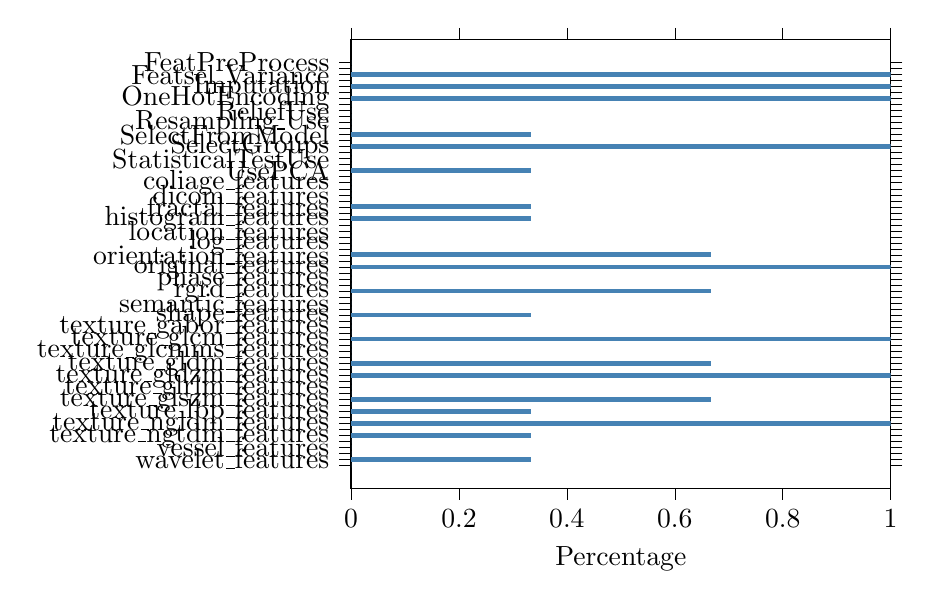
\begin{tikzpicture}

\definecolor{color0}{rgb}{0.274509803921569,0.509803921568627,0.705882352941177}

\begin{axis}[
tick align=outside,
tick pos=both,
x grid style={white!69.0196078431373!black},
xlabel={Percentage},
xmin=0, xmax=1,
xtick style={color=black},
y dir=reverse,
y grid style={white!69.0196078431373!black},
ymin=-3.79, ymax=70.79,
ytick style={color=black},
ytick={0,1,2,3,4,5,6,7,8,9,10,11,12,13,14,15,16,17,18,19,20,21,22,23,24,25,26,27,28,29,30,31,32,33,34,35,36,37,38,39,40,41,42,43,44,45,46,47,48,49,50,51,52,53,54,55,56,57,58,59,60,61,62,63,64,65,66,67},
yticklabels={FeatPreProcess,,Featsel\_Variance,,Imputation,,OneHotEncoding,,ReliefUse,,Resampling\_Use,,SelectFromModel,,SelectGroups,,StatisticalTestUse,,UsePCA,,coliage\_features,,dicom\_features,,fractal\_features,,histogram\_features,,location\_features,,log\_features,,orientation\_features,,original\_features,,phase\_features,,rgrd\_features,,semantic\_features,,shape\_features,,texture\_gabor\_features,,texture\_glcm\_features,,texture\_glcmms\_features,,texture\_gldm\_features,,texture\_gldzm\_features,,texture\_glrlm\_features,,texture\_glszm\_features,,texture\_lbp\_features,,texture\_ngldm\_features,,texture\_ngtdm\_features,,vessel\_features,,wavelet\_features,}
]
\draw[draw=none,fill=color0] (axis cs:0,-0.4) rectangle (axis cs:0,0.4);
\draw[draw=none,fill=color0] (axis cs:0,0.6) rectangle (axis cs:0,1.4);
\draw[draw=none,fill=color0] (axis cs:0,1.6) rectangle (axis cs:1,2.4);
\draw[draw=none,fill=color0] (axis cs:0,2.6) rectangle (axis cs:0,3.4);
\draw[draw=none,fill=color0] (axis cs:0,3.6) rectangle (axis cs:1,4.4);
\draw[draw=none,fill=color0] (axis cs:0,4.6) rectangle (axis cs:0,5.4);
\draw[draw=none,fill=color0] (axis cs:0,5.6) rectangle (axis cs:1,6.4);
\draw[draw=none,fill=color0] (axis cs:0,6.6) rectangle (axis cs:0,7.4);
\draw[draw=none,fill=color0] (axis cs:0,7.6) rectangle (axis cs:0,8.4);
\draw[draw=none,fill=color0] (axis cs:0,8.6) rectangle (axis cs:0,9.4);
\draw[draw=none,fill=color0] (axis cs:0,9.6) rectangle (axis cs:0,10.4);
\draw[draw=none,fill=color0] (axis cs:0,10.6) rectangle (axis cs:0,11.4);
\draw[draw=none,fill=color0] (axis cs:0,11.6) rectangle (axis cs:0.333333333333333,12.4);
\draw[draw=none,fill=color0] (axis cs:0,12.6) rectangle (axis cs:0,13.4);
\draw[draw=none,fill=color0] (axis cs:0,13.6) rectangle (axis cs:1,14.4);
\draw[draw=none,fill=color0] (axis cs:0,14.6) rectangle (axis cs:0,15.4);
\draw[draw=none,fill=color0] (axis cs:0,15.6) rectangle (axis cs:0,16.4);
\draw[draw=none,fill=color0] (axis cs:0,16.6) rectangle (axis cs:0,17.4);
\draw[draw=none,fill=color0] (axis cs:0,17.6) rectangle (axis cs:0.333333333333333,18.4);
\draw[draw=none,fill=color0] (axis cs:0,18.6) rectangle (axis cs:0,19.4);
\draw[draw=none,fill=color0] (axis cs:0,19.6) rectangle (axis cs:0,20.4);
\draw[draw=none,fill=color0] (axis cs:0,20.6) rectangle (axis cs:0,21.4);
\draw[draw=none,fill=color0] (axis cs:0,21.6) rectangle (axis cs:0,22.4);
\draw[draw=none,fill=color0] (axis cs:0,22.6) rectangle (axis cs:0,23.4);
\draw[draw=none,fill=color0] (axis cs:0,23.6) rectangle (axis cs:0.333333333333333,24.4);
\draw[draw=none,fill=color0] (axis cs:0,24.6) rectangle (axis cs:0,25.4);
\draw[draw=none,fill=color0] (axis cs:0,25.6) rectangle (axis cs:0.333333333333333,26.4);
\draw[draw=none,fill=color0] (axis cs:0,26.6) rectangle (axis cs:0,27.4);
\draw[draw=none,fill=color0] (axis cs:0,27.6) rectangle (axis cs:0,28.4);
\draw[draw=none,fill=color0] (axis cs:0,28.6) rectangle (axis cs:0,29.4);
\draw[draw=none,fill=color0] (axis cs:0,29.6) rectangle (axis cs:0,30.4);
\draw[draw=none,fill=color0] (axis cs:0,30.6) rectangle (axis cs:0,31.4);
\draw[draw=none,fill=color0] (axis cs:0,31.6) rectangle (axis cs:0.666666666666667,32.4);
\draw[draw=none,fill=color0] (axis cs:0,32.6) rectangle (axis cs:0,33.4);
\draw[draw=none,fill=color0] (axis cs:0,33.6) rectangle (axis cs:1,34.4);
\draw[draw=none,fill=color0] (axis cs:0,34.6) rectangle (axis cs:0,35.4);
\draw[draw=none,fill=color0] (axis cs:0,35.6) rectangle (axis cs:0,36.4);
\draw[draw=none,fill=color0] (axis cs:0,36.6) rectangle (axis cs:0,37.4);
\draw[draw=none,fill=color0] (axis cs:0,37.6) rectangle (axis cs:0.666666666666667,38.4);
\draw[draw=none,fill=color0] (axis cs:0,38.6) rectangle (axis cs:0,39.4);
\draw[draw=none,fill=color0] (axis cs:0,39.6) rectangle (axis cs:0,40.4);
\draw[draw=none,fill=color0] (axis cs:0,40.6) rectangle (axis cs:0,41.4);
\draw[draw=none,fill=color0] (axis cs:0,41.6) rectangle (axis cs:0.333333333333333,42.4);
\draw[draw=none,fill=color0] (axis cs:0,42.6) rectangle (axis cs:0,43.4);
\draw[draw=none,fill=color0] (axis cs:0,43.6) rectangle (axis cs:0,44.4);
\draw[draw=none,fill=color0] (axis cs:0,44.6) rectangle (axis cs:0,45.4);
\draw[draw=none,fill=color0] (axis cs:0,45.6) rectangle (axis cs:1,46.4);
\draw[draw=none,fill=color0] (axis cs:0,46.6) rectangle (axis cs:0,47.4);
\draw[draw=none,fill=color0] (axis cs:0,47.6) rectangle (axis cs:0,48.4);
\draw[draw=none,fill=color0] (axis cs:0,48.6) rectangle (axis cs:0,49.4);
\draw[draw=none,fill=color0] (axis cs:0,49.6) rectangle (axis cs:0.666666666666667,50.4);
\draw[draw=none,fill=color0] (axis cs:0,50.6) rectangle (axis cs:0,51.4);
\draw[draw=none,fill=color0] (axis cs:0,51.6) rectangle (axis cs:1,52.4);
\draw[draw=none,fill=color0] (axis cs:0,52.6) rectangle (axis cs:0,53.4);
\draw[draw=none,fill=color0] (axis cs:0,53.6) rectangle (axis cs:0,54.4);
\draw[draw=none,fill=color0] (axis cs:0,54.6) rectangle (axis cs:0,55.4);
\draw[draw=none,fill=color0] (axis cs:0,55.6) rectangle (axis cs:0.666666666666667,56.4);
\draw[draw=none,fill=color0] (axis cs:0,56.6) rectangle (axis cs:0,57.4);
\draw[draw=none,fill=color0] (axis cs:0,57.6) rectangle (axis cs:0.333333333333333,58.4);
\draw[draw=none,fill=color0] (axis cs:0,58.6) rectangle (axis cs:0,59.4);
\draw[draw=none,fill=color0] (axis cs:0,59.6) rectangle (axis cs:1,60.4);
\draw[draw=none,fill=color0] (axis cs:0,60.6) rectangle (axis cs:0,61.4);
\draw[draw=none,fill=color0] (axis cs:0,61.6) rectangle (axis cs:0.333333333333333,62.4);
\draw[draw=none,fill=color0] (axis cs:0,62.6) rectangle (axis cs:0,63.4);
\draw[draw=none,fill=color0] (axis cs:0,63.6) rectangle (axis cs:0,64.4);
\draw[draw=none,fill=color0] (axis cs:0,64.6) rectangle (axis cs:0,65.4);
\draw[draw=none,fill=color0] (axis cs:0,65.6) rectangle (axis cs:0.333333333333333,66.4);
\draw[draw=none,fill=color0] (axis cs:0,66.6) rectangle (axis cs:0,67.4);
\end{axis}

\end{tikzpicture}
